\begin{frame}
    \frametitle{Run time}
    Explicit run time data was not collected, but based on the file timestamps,
    we can estimate how long each case took to complete on a cluster
    \begin{table}[htpb]
        \centering
        \caption{Comparison of average total runtimes}
        \label{tab:label}
        \begin{tabular}{|c|c|p{0.5\linewidth}|}
         Case & Runtime scale & Notes\\
         1 & hours &  \\
         2 & minutes & Does not include the initial simulation to obatin $\phi_{g}$
         and $\sigma_{i,g}$ \\
         3 & hours & Cross section data had to be loaded in at each timestep, s
         this case took the longest amount of time
        \end{tabular}
    \end{table}
    Case 2 is {\it very} fast!
\end{frame}

\begin{frame}
    \frametitle{One-group actinides (3-day time steps)}
    \begin{figure}[htpb]
        \centering
        \subfloat[] {
            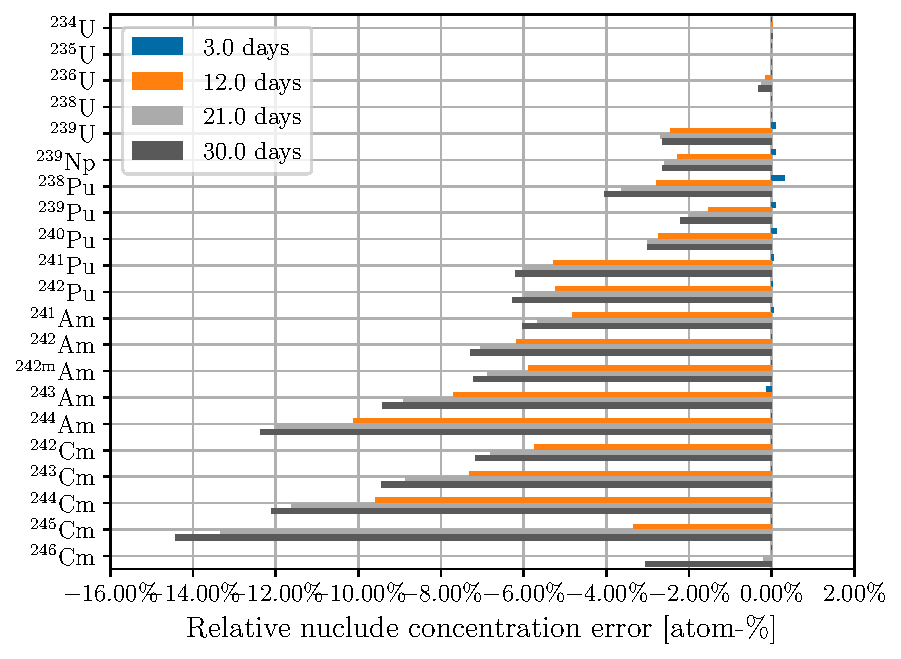
\includegraphics[width=0.5\linewidth]{./../paper/figs/actinides_constant_xs_predictor_fission_q_days.pdf}
            \label{fig:actinides-error-constant-xs-days}
        }
        \subfloat[] {
            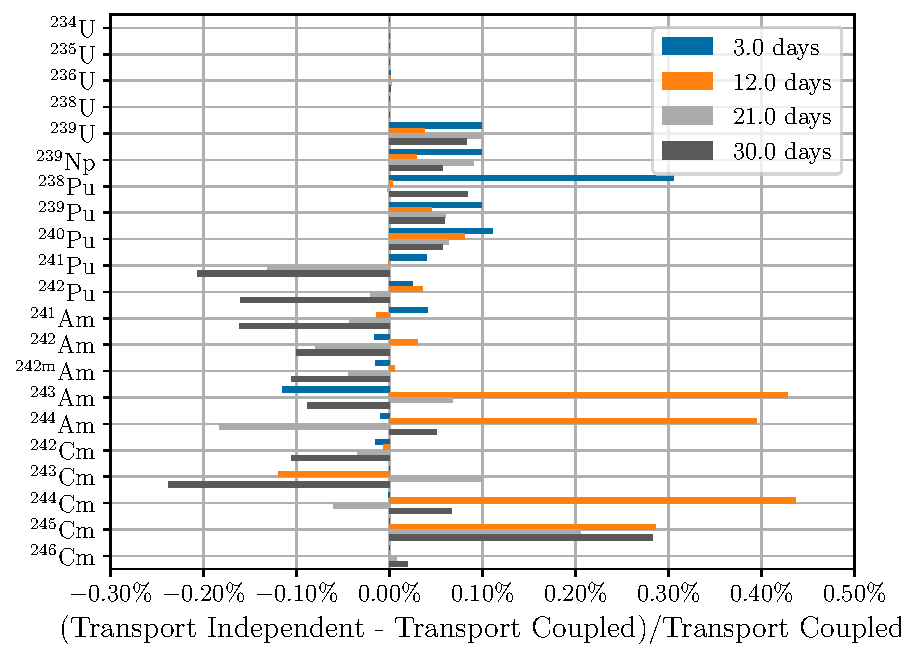
\includegraphics[width=0.5\linewidth]{./../paper/figs/actinides_updating_xs_predictor_fission_q_days.pdf}
            \label{fig:actinides-error-updating-xs-days}
        }
        \caption[]{Actinide concentration error relative to Case 1 using 3-day time steps at 3,
                12, 21, and 30 days of depletion for
            \subref{fig:actinides-error-constant-xs-days} constant cross
            sections (Case 2);
            \subref{fig:actinides-error-updating-xs-days} updating cross
            sections (Case 3).}
    \end{figure}
\end{frame}

\begin{frame}
    \frametitle{One-group actinides (30-day time steps)}
    \begin{figure}[h!tpb]
        \centering
        \subfloat[] {
            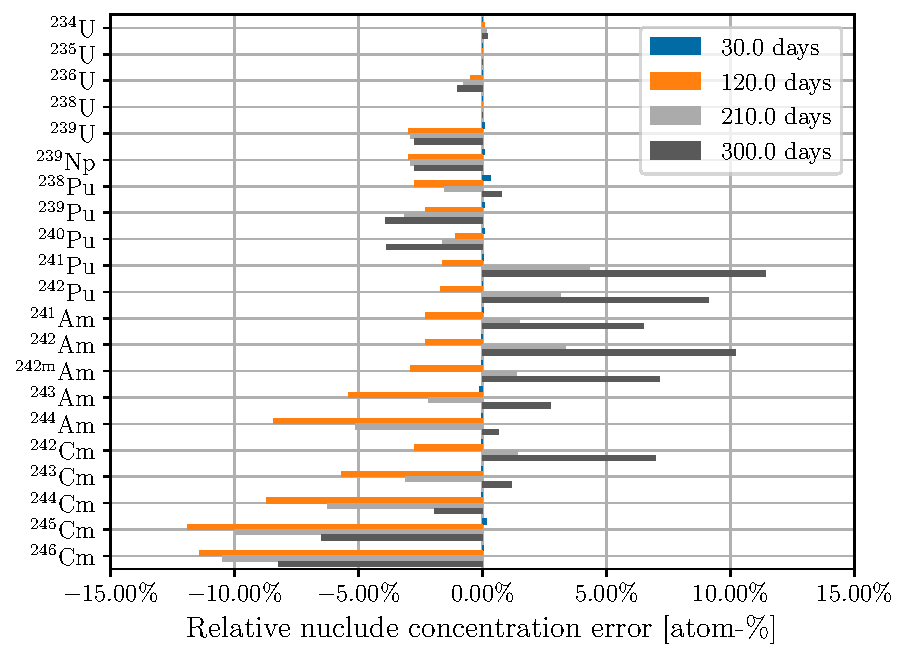
\includegraphics[width=0.5\linewidth]{./../paper/figs/actinides_constant_xs_predictor_fission_q_months.pdf}
            \label{fig:actinides-error-constant-xs-months}
        }
        \subfloat[] {
            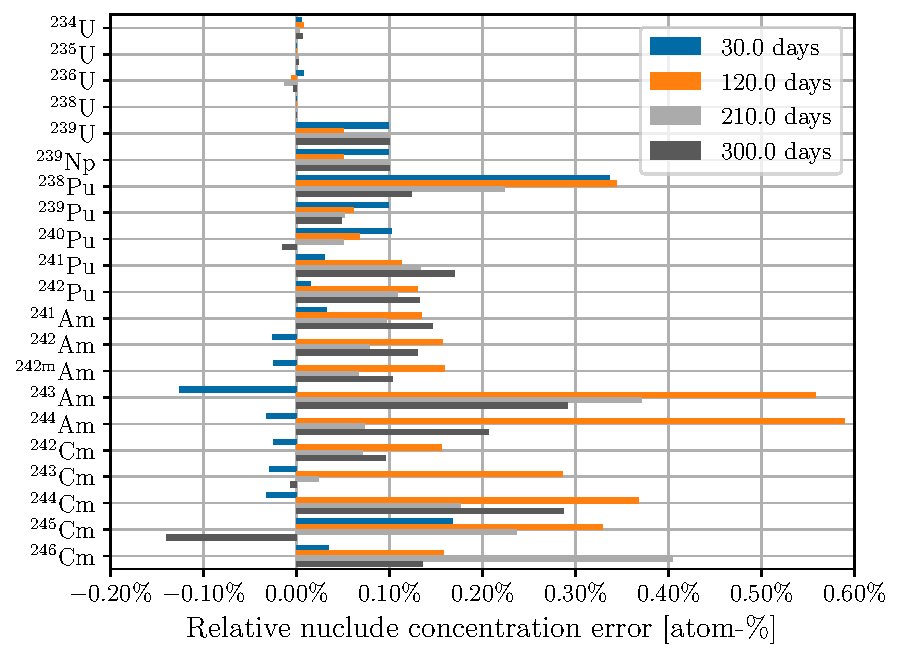
\includegraphics[width=0.5\linewidth]{./../paper/figs/actinides_updating_xs_predictor_fission_q_months.pdf}
            \label{fig:actinides-error-updating-xs-months}
        }
        \caption[]{Actinide concentration error relative to Case 1 using 30-day time steps
            at 30,
                120, 210, and 300 months of depletion for
            \subref{fig:actinides-error-constant-xs-months} constant cross
            sections (Case 2);
            \subref{fig:actinides-error-updating-xs-months} updating cross
            sections (Case 3).}
    \end{figure}
\end{frame}

\begin{frame}
    \frametitle{Overprediction of $(n,\gamma)$ reaction rates on \ce{^{240}Pu}}
    \begin{figure}[htpb]
        \centering
        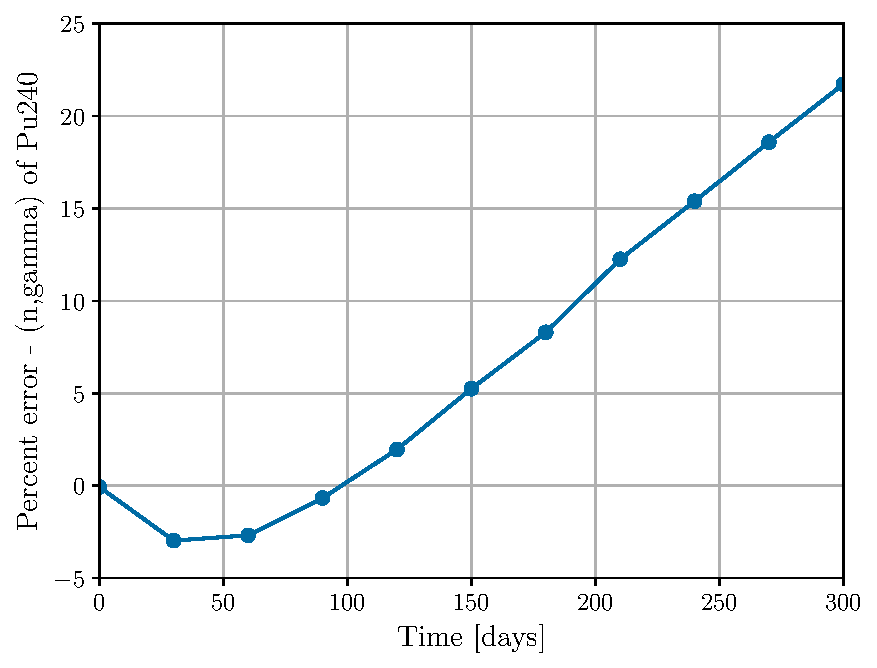
\includegraphics[width=0.5\linewidth]{./../paper/figs/pu240-n-gamma-months.pdf}
        \caption{Relative \ce{^{240}Pu} ($n,\gamma$) reaction rate error using
        constant cross sections and 30-day time steps.}
        \label{fig:pu240-n-gamma-months}
    \end{figure}
\end{frame}



\begin{frame}
    \frametitle{Fission products (3-day time steps)}
    \begin{figure}[h!tpb]
        \centering
        \subfloat[] {
            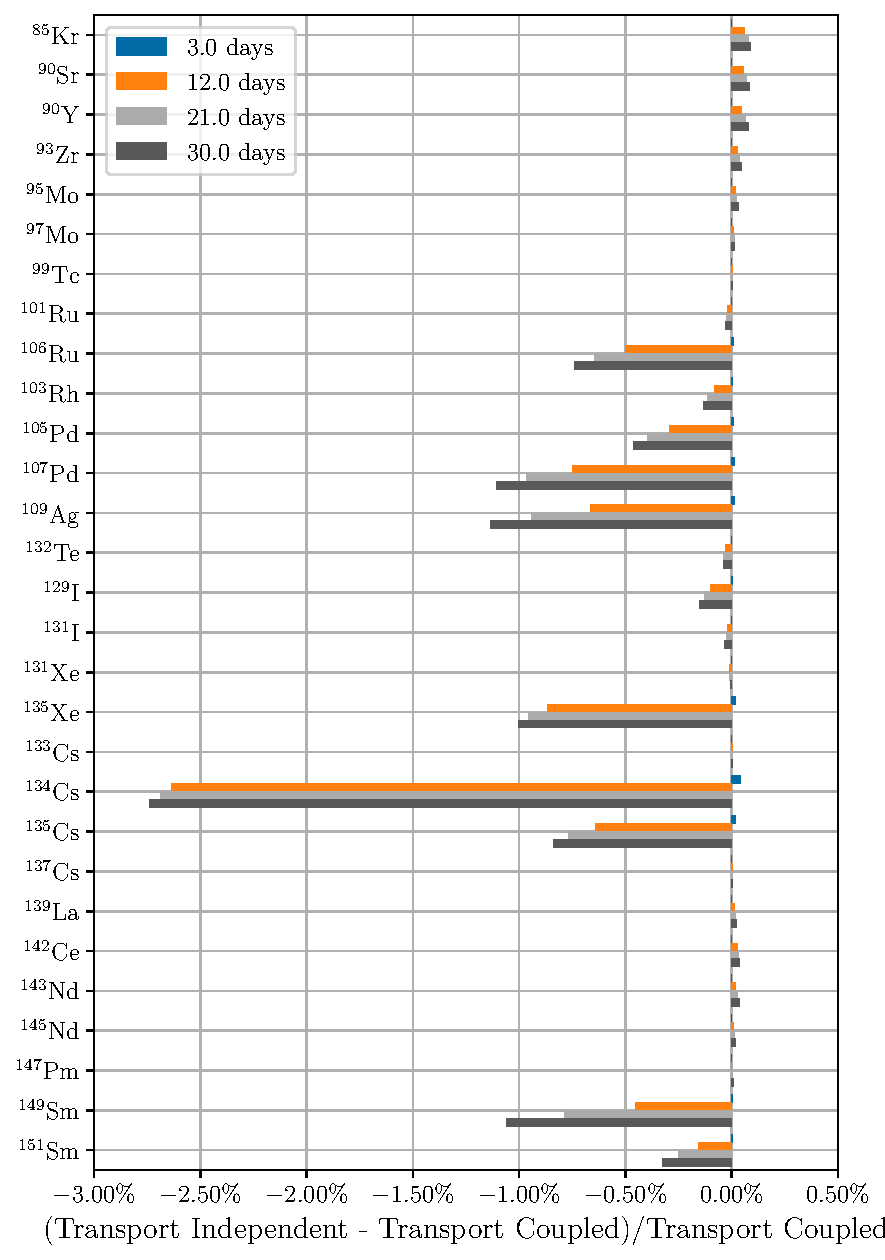
\includegraphics[width=0.4\linewidth]{./../paper/figs/fission_products_constant_xs_predictor_fission_q_days.pdf}
            \label{fig:fp-error-constant-xs-days}
        }
        \subfloat[] {
            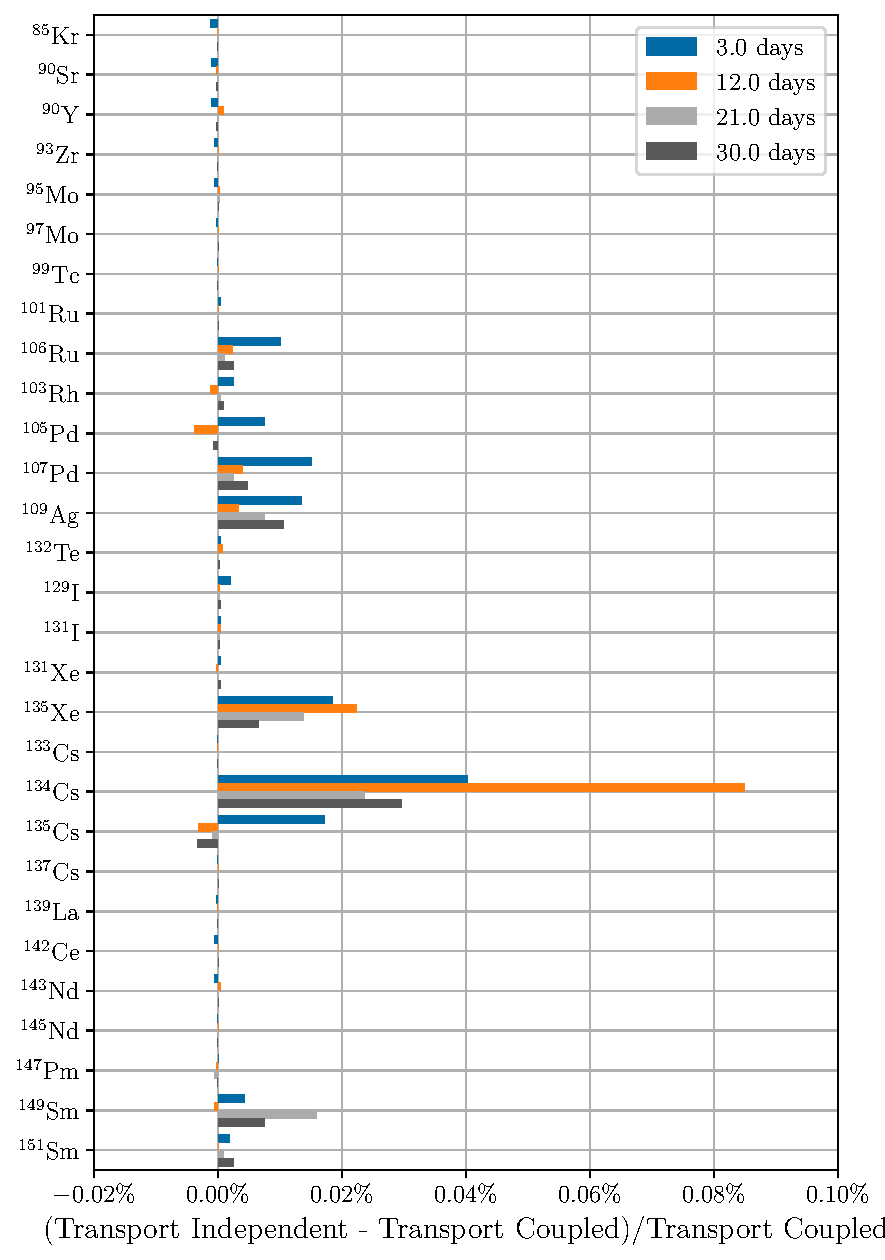
\includegraphics[width=0.4\linewidth]{./../paper/figs/fission_products_updating_xs_predictor_fission_q_days.pdf}
            \label{fig:fp-error-updating-xs-days}
        }
        \caption[]{\subref{fig:fp-error-constant-xs-days} constant cross
            sections (Case 2);
            \subref{fig:fp-error-updating-xs-days} updating cross sections (Case
        3).}
    \end{figure}
\end{frame}

\begin{frame}
    \frametitle{Fission products (30-day time steps)}
    \begin{figure}[h!tpb]
        \centering
        \subfloat[] {
            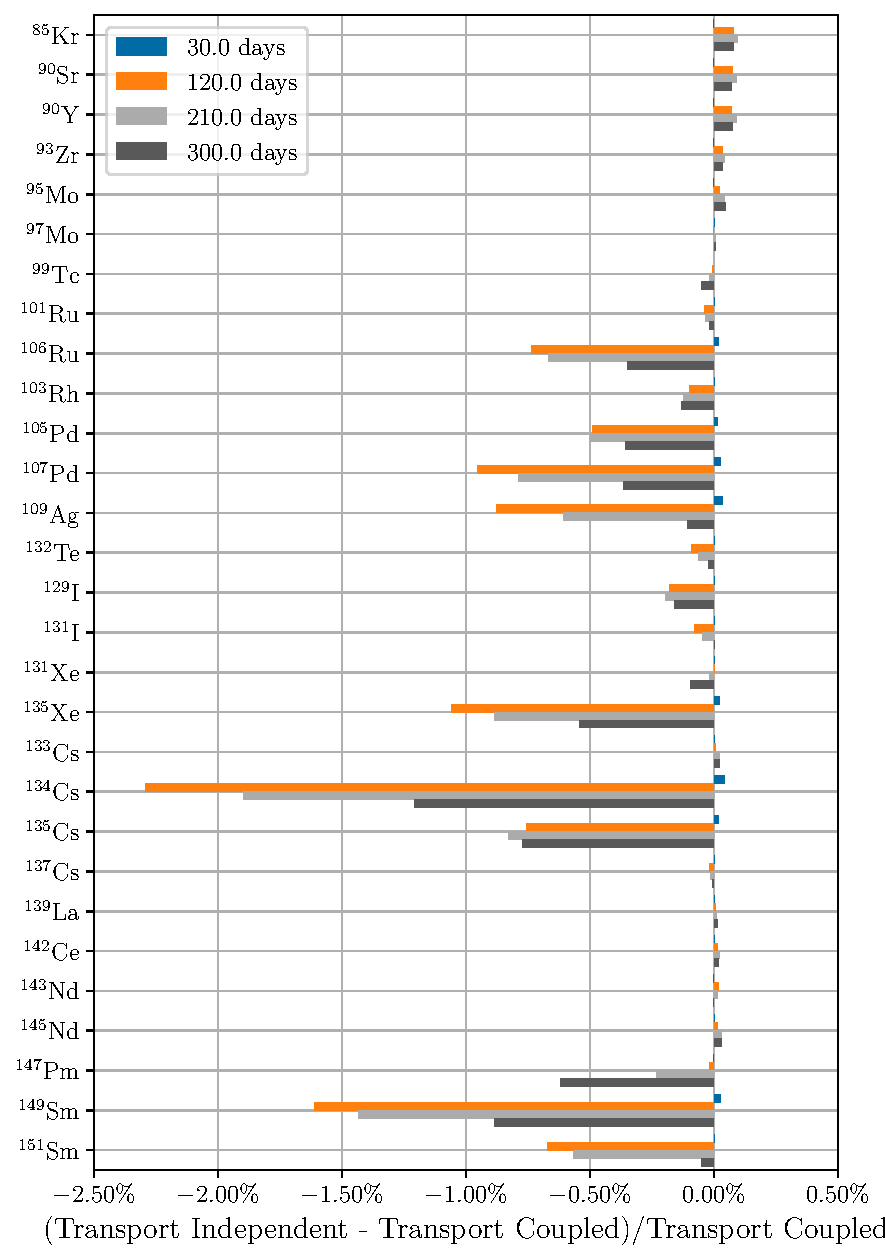
\includegraphics[width=0.4\linewidth]{./../paper/figs/fission_products_constant_xs_predictor_fission_q_months.pdf}
            \label{fig:fp-error-constant-xs-months}
        }
        \subfloat[] {
            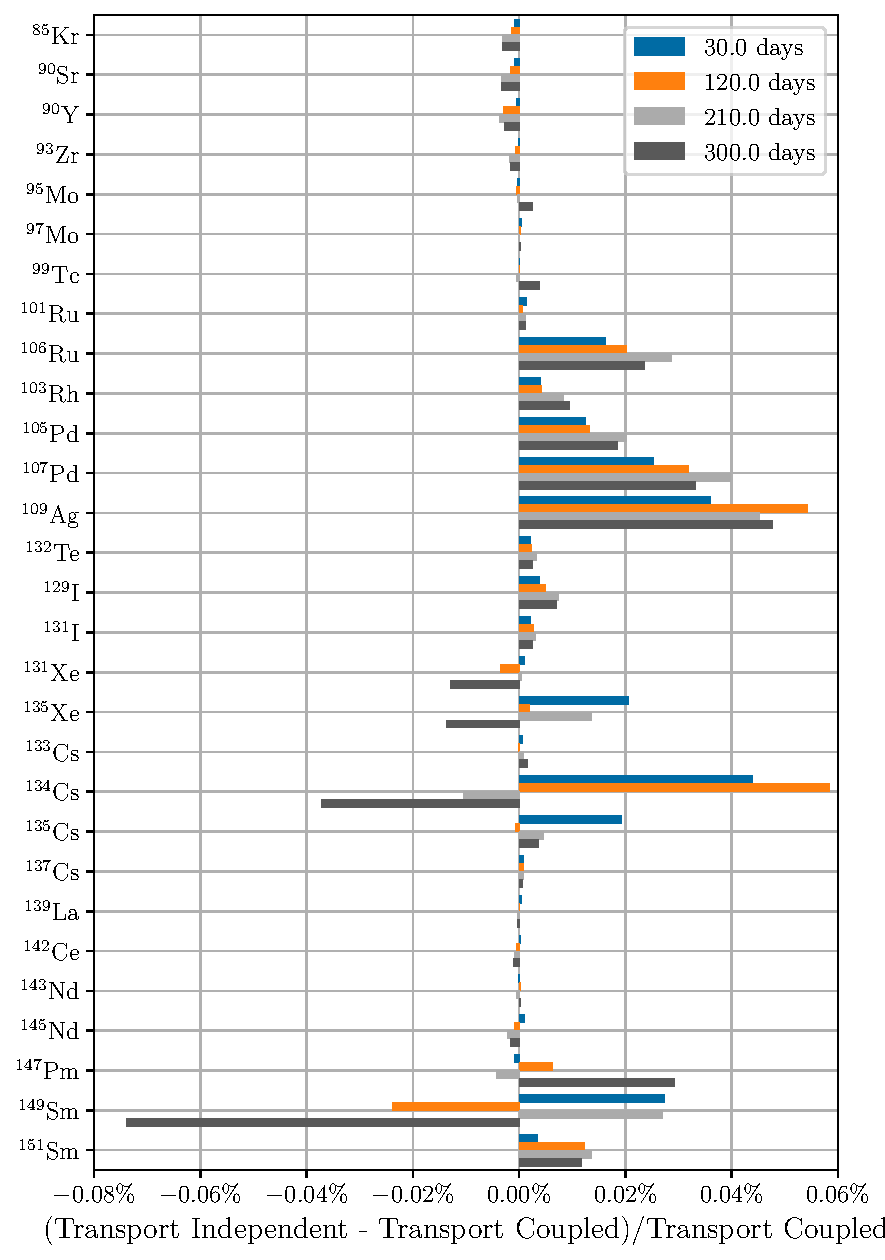
\includegraphics[width=0.4\linewidth]{./../paper/figs/fission_products_updating_xs_predictor_fission_q_months.pdf}
            \label{fig:fp-error-updating-xs-months}
        }
        \caption[]{\subref{fig:fp-error-constant-xs-months} constant cross
            sections (Case 2);
            \subref{fig:fp-error-updating-xs-months} updating cross sections
        (Case 3).}
    \end{figure}
\end{frame}

\begin{frame}
    \frametitle{8-group actinides}
    \begin{figure}[htpb]
        \centering
        \subfloat[] {
            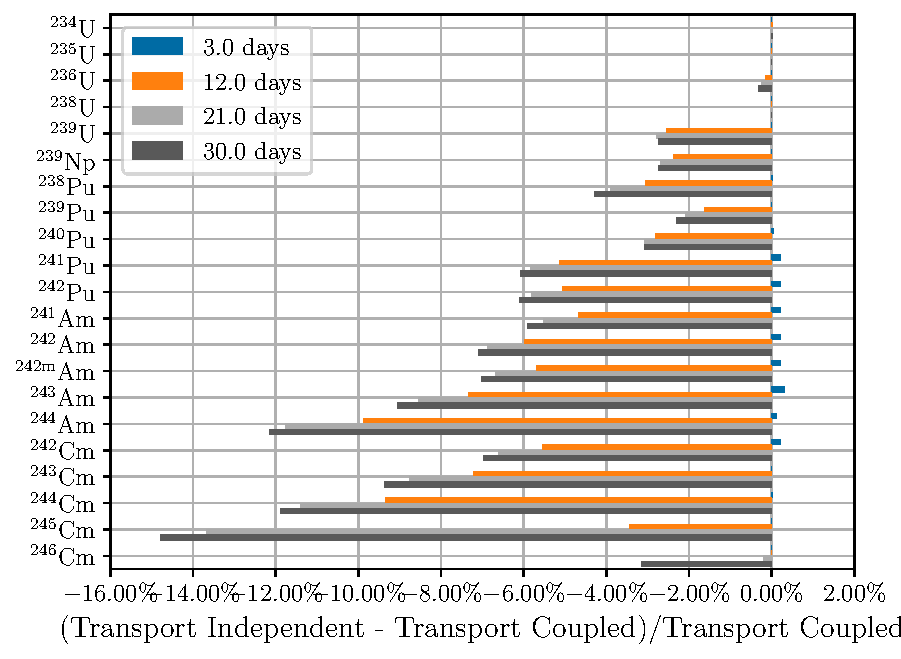
\includegraphics[width=0.5\linewidth]{./../paper/figs/actinides_casmo8_constant_xs_predictor_fission_q_days.pdf}
            \label{fig:actinides-error-casmo8-xs-days}
        }
        \subfloat[] {
            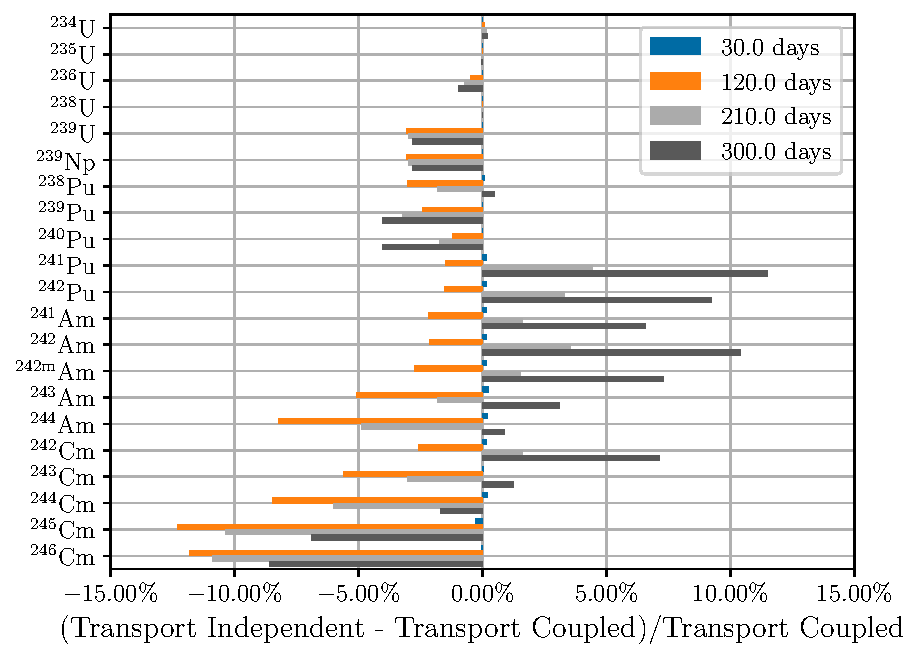
\includegraphics[width=0.5\linewidth]{./../paper/figs/actinides_casmo8_constant_xs_predictor_fission_q_months.pdf}
            \label{fig:actinides-error-casmo8-xs-months}
        }
        \caption[]{
            \subref{fig:actinides-error-casmo8-xs-days} 3-day time steps;
            \subref{fig:actinides-error-casmo8-xs-months} 30-day time steps}
    \end{figure}
\end{frame}

\begin{frame}
    \frametitle{40-group actinides}
    \begin{figure}[htpb]
        \centering
        \subfloat[] {
            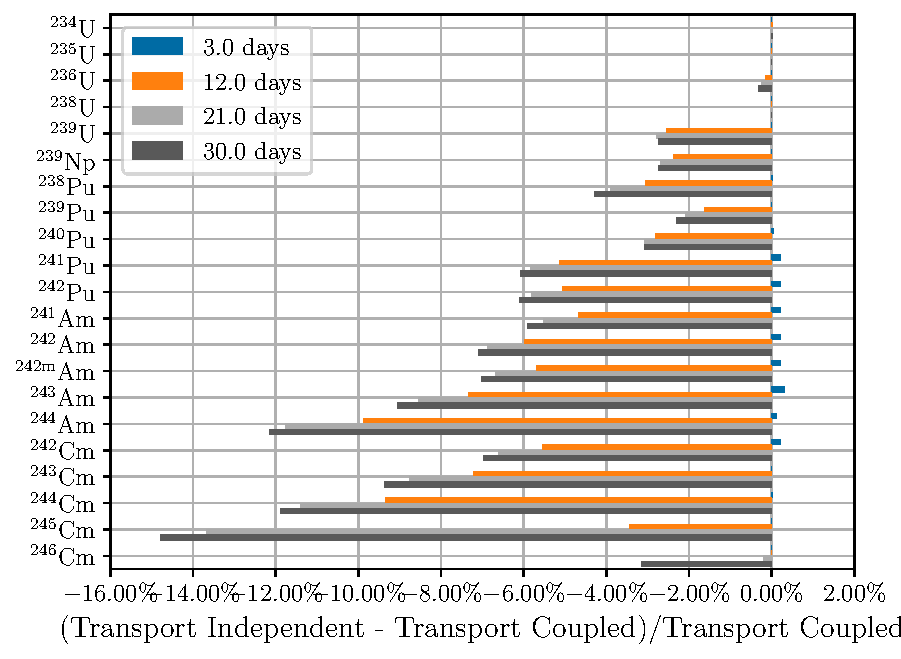
\includegraphics[width=0.5\linewidth]{./../paper/figs/actinides_casmo40_constant_xs_predictor_fission_q_days.pdf}
            \label{fig:actinides-error-casmo40-xs-days}
        }
        \subfloat[] {
            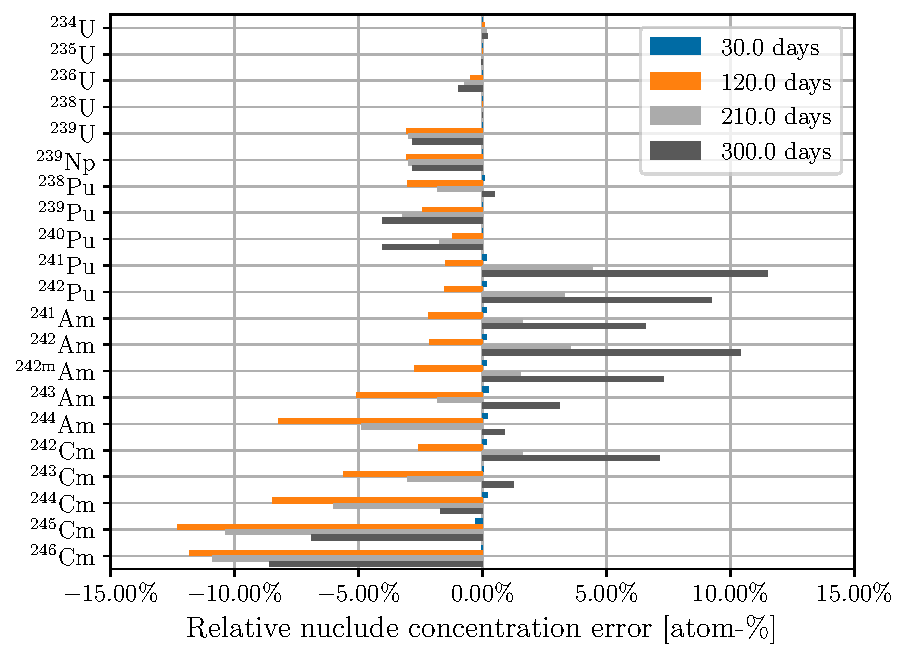
\includegraphics[width=0.5\linewidth]{./../paper/figs/actinides_casmo40_constant_xs_predictor_fission_q_months.pdf}
            \label{fig:actinides-error-casmo40-xs-months}
        }
        \caption[]{
            \subref{fig:actinides-error-casmo40-xs-days} 3-day time steps;
            \subref{fig:actinides-error-casmo40-xs-months} 30-day time steps}
    \end{figure}
\end{frame}
